\chapter{ECG's standard deviation estimation using a Convolutional Neural
Network}\label{ch:cnn}

In this chapter I will discuss the design and implementation of a convolutional
neural network used to estimate the standard deviation of the ECG signal, since
the MLP developed in \chref{ch:ecg} performed poorly. This implements the
requirements for the Task 4.1 of the Project Specifications.

For this task, I've modified (through the use of some parameters) how the
\code{augmentdata} stage perform the data augmentation on the dataset. All the
samples extracted via random subsampling are now all of the same length (2500
time steps, or 5 seconds).

In the following sections, I'm going to run the training of different CNN
architectures in order to try to find a good architecture. CNN definitions can
be found in directory \code{src/cnndefs}, where each file has a name in the
form \code{cnndefX.m}, where \(X\) is an incremental number. So, when in the
text I refer, for example, to the ``CNN definition 7'', you can see the
architecture in \code{src/cnndefs/cnndef7.m}.

Moreover, directory \code{diaries} contains the diaries of execution of all
tested architectures. Here, you can find all the results in the last lines of
each file named \code{cnntrain\_cnndefX.txt}.

The training of a CNN, can be run with:
\begin{verbatim}
> cnntrain X
\end{verbatim}
where \(X\) is the CNN definition number. If not specified, it will run the
training of the final CNN architecture\footnote{In file
\code{src/cnndefs/cnndef.m}.}.

Other parameters can be specified, for example:
\begin{verbatim}
> cnntrain(15, 'epochs', 20, 'valRatio', 0.15, ...
        'testRatio', 0.15)
\end{verbatim}
will run the training of CNN definition 15 with 20 epochs using also a
validation and a test set.

The script \code{cnntrain} is in the \code{src/scripts} folder, as usual.

\section{Selection of the base block of the CNN}\label{sec:cnnbase}

I will start with the CNN definition shown in \lstref{lst:cnndef1}.

\lstinputlisting[language={matlab}, label={lst:cnndef1}, style={Matlab-editor},
basicstyle={\footnotesize\ttfamily}, caption={\code{cnndef1.m}}]{cnndef1.m}

The base block of the CNN is:
\begin{enumerate}
	\item A \standout{1-dimensional convolutional layer} with 16 filters,
		with each filter of size 5. The filters will slide over the
		input with a stride of 2.
	\item A \standout{batch normalization layer}. Used between every
		convolutional layer and non-linear layers, as recommended by
		the MATLAB documentation, in order to speed up the training
		process and reduce the sensitivity to network initialization.
	\item A \standout{leaky ReLU layer}, to avoid the vanishing gradient
		issue.
	\item A \standout{max pooling layer} of size 3 and with a stride of 2.
\end{enumerate}

After the base block, the architecture has a \standout{global average pooling
layer} and then some \standout{fully connected layers}.

In this section, I will try to optimize this base block by trying to change
various parameters. Note that I will just use a training set for these tests,
as the periodic validation of the validation set by the training algorithm
causes a huge slow down in the training process.

\subsection{Size of filters and stride}

I will start with the size of filters of the convolutional layer and their
stride. CNN definitions from 1 to 14 try different combinations of these
parameters. \tableref{table:cnnfiltersizestride} contains the results obtained
from some of the tests done\footnote{I will report here only the most
interesting results. Results of other runs can be found in diaries.}. For each
run:
\begin{itemize}
	\item The first column contains the definition number of the CNN.
	\item The second column contains the parameters used. The first number
		is the size of the filters, while the second number is the
		value used for the stride.
	\item The third column contains the RMSE (Root Mean Square Error) of
		the CNN at the last iteration.
	\item The fourth column is the RMSE of the CNN at the \emph{best}
		iteration \idest{the one for which the loss function returned
		the lowest value}. When I will train the final CNN, I will use
		also a validation set and I will stop the training when the
		validation error stops decreasing --- so this value may be
		considered as an estimate of the result that I may obtain with
		the validation set.
	\item The last column is the correlation coefficient (\(R\)) to
		evaluate the regression quality.
\end{itemize}

\begin{table}[hbtp]
	\centering
	\begin{tabular}{|c|c|c|c|c|}
		\toprule
		\# & Params & RMSE & Best RMSE & R \\
		\midrule
		4 & 15, 4 & \(948.81\) & \(664.15\) & \(0.758\) \\
		5 & 25, 4 & \(1377.5\) & \(541.93\) & \(0.751\) \\
		7 & 9, 3 & \(2013.3\) & \(514.46\) & \(0.748\) \\
		7\emph{bis} & 9, 3 & \(680.05\) & \(655.85\) & \(0.757\) \\
		11 & 7, 2 & \(955.2\) & \(651.47\) & \(0.752\) \\
		13 & 11, 2 & \(665.53\) & \(783.15\) & \(0.755\) \\
		\bottomrule
	\end{tabular}
	\caption{Some (not all) of the results obtained in the attempt to
	optimize the size and the stride of the filters of the convolutional
	layer. Note that \code{cnndef7} has been executed 2
	times.}\label{table:cnnfiltersizestride}
\end{table}

Based on the results, I will use a filter size of 9 and a stride of 3
(\code{cnndef7}). It is the second best result according to the \(R\)
parameter, but it is the first one according to the RMSE of the best iteration
(\(514.46\)).

\subsection{Type of pooling layers}

Using the architecture of \code{cnndef7} as a base, the CNN definitions from 15
to 17 try different combinations for the types of pooling layers (the pooling
layer at the output of the base convolutional block and the global pooling
layer before the fully connected layers).

Results in \tableref{table:cnnpoolingtypes}. For the ``Params'' column, the
first is the type of the pooling layer of the convolutional block, while the
second is the type of the global pooling layer.

\begin{table}[hbtp]
	\centering
	\begin{tabular}{|c|c|c|c|c|}
		\toprule
		\# & Params & RMSE & Best RMSE & R \\
		\midrule
		7 & max, avg & \(2013.3\) & \(514.46\) & \(0.748\) \\
		7\emph{bis} & max, avg & \(680.05\) & \(655.85\) & \(0.757\) \\
		15 & avg, avg & \(708.32\) & \(631.68\) & \(0.751\) \\
		16 & avg, max & \(1049.09\) & \(879.13\) & \(0.511\) \\
		17 & max, max & \(1180.54\) & \(786.54\) & \(0.610\) \\
		\bottomrule
	\end{tabular}
	\caption{Trying different combinations for the type of pooling
	layers.}\label{table:cnnpoolingtypes}
\end{table}

Based on the results, I will use \code{maxPooling1dLayer} for the convolutional
block and \code{globalAveragePooling1dLayer} before the fully connected layers,
as I was doing before.

\subsection{Size of pooling regions and stride}

CNN definitions from 18 to 21 try different combinations for the size of
pooling regions for the \code{maxPooling1dLayer} and its stride. I will not
show the results here (check the diaries if interested): I will just say that
the values which gave the best results are 3 for the size of the regions and 2
for the stride.

\subsection{Final CNN base block}\label{subsec:cnnfinalbase}

Using \code{cnndef22} I have also tried to change the padding mode of the
convolutional layer from ``same'' to ``causal'', but it achieved lower
performances.

So, the final selected CNN base block is shown in \lstref{lst:cnndef7}. This
block will be used in the following sections to build a more complex CNN
architecture.

\lstinputlisting[language={matlab}, label={lst:cnndef7}, style={Matlab-editor},
basicstyle={\footnotesize\ttfamily}, caption={Optimized CNN convolutional base
block.}]{cnndef7.m}

\section{Selection of the number of convolutional
layers}\label{sec:cnnconvlayers}

CNN definitions from 23 to 26 try different architectures by increasing the
number of convolutional blocks. Each block has the same structure, as defined
in \secref{subsec:cnnfinalbase}. Note that now the number of filters of a
convolutional layer is computed as \(i\times16\), where \(i\) is an integer
which increases going down in the CNN, so that the first convolutional layer
has 16 filters; the second has 32 filters; the third has 48 filters and so on.
As we move forward through layers, the patterns that the convolutional layers
must try to identify become more complex and more filters may allow the network
to better find these patterns.

To account for the increased number of filters in the last convolutional layer,
I've also increased the size of fully connected layers. Since now the
architecture is quite complex, I am also going to perform tests using 60 epochs
(instead of 30, as before).

Results in \tableref{table:cnnconvlayers}. The best results are given by the
last 2 CNNs, with 4 and 5 convolutional blocks.

\begin{table}[hbtp]
	\centering
	\begin{tabular}{|c|c|c|c|c|}
		\toprule
		\# & Layers & RMSE & Best RMSE & R \\
		\midrule
		7 (30 epochs) & 1 & \(2013.3\) & \(514.46\) & \(0.748\) \\
		7\emph{bis} (30 epochs) & 1 & \(680.05\) & \(655.85\) & \(0.757\) \\
		23 & 2 & \(467.33\) & \(413.65\) & \(0.915\) \\
		24 & 3 & \(466.06\) & \(335.28\) & \(0.935\) \\
		25 & 4 & \(382.39\) & \(406.14\) & \(0.940\) \\
		26 & 5 & \(500.22\) & \(243.24\) & \(0.939\) \\
		\bottomrule
	\end{tabular}
	\caption{Increasing the number of convolutional
	blocks.}\label{table:cnnconvlayers}
\end{table}

\section{Selection of the number of filters}\label{sec:cnnfilters}

Here I will try to increase the number of filters by tuning the \code{nf}
parameter. This parameter is multiplied with the ``depth'' of the convolutional
layer to obtain the number of filters in the layer. Some of the test will use 4
convolutional layers; others will use 5 convolutional layers.

Results in \tableref{table:cnnfilters}. The most complex architecture tested,
with 5 convolutional layers and \code{nf = 64}, is the best one.

\begin{table}[hbtp]
	\centering
	\begin{tabular}{|c|c|c|c|}
		\toprule
		\# & Layers & nf & R \\
		\midrule
		25 & 4 & 16 & \(0.940\) \\
		26 & 5 & 16 & \(0.939\) \\
		27 & 4 & 32 & \(0.944\) \\
		28 & 4 & 48 & \(0.947\) \\
		29 & 4 & 64 & \(0.945\) \\
		30 & 5 & 32 & \(0.946\) \\
		31 & 5 & 48 & \(0.946\) \\
		32 & 5 & 64 & \(0.949\) \\
		\bottomrule
	\end{tabular}
	\caption{Increasing the number of filters. Only the \(R\) parameter is
	reported.}\label{table:cnnfilters}
\end{table}

\section{Testing of other CNN architectures}\label{sec:cnnarch}

I've tested other architectures, by trying to change:
\begin{itemize}
	\item The size of the filters in each convolutional layer, even by
		using different sizes for different layers.
	\item The size of the pooling layers (different sizes for different
		layers).
	\item The stride of the last pooling layers.
\end{itemize}

This has been done using the CNN definitions from 33 to 35. None of them have
outperfomed the CNN architecture defined in \secref{sec:cnnfilters}.

\section{Selection of the normalization algorithm}\label{sec:rnnnormalization}

I've tried all possible choices for the normalization algorithm for the input
sequences. Results in \tableref{table:rnnnormalization}.

\begin{table}[hbtp]
	\centering
	\begin{tabular}{|c|c|c|c|}
		\toprule
		\# & Normalization algorithm & RMSE & Best RMSE \\
		\midrule
		1 & \code{rescale-symmetric} & \(6128.04\) & \(3087.69\) \\
		11 & \code{zerocenter} & \(13938.16\) & \(11285.47\) \\
		12 & \code{zscore} & \(3157.22\) & \(2930.36\) \\
		13 & \code{rescale-zero-one} & \(10997.16\) & \(10982.06\) \\
		\bottomrule
	\end{tabular}
	\caption{Changing the normalization algorithm for the
	RNN.}\label{table:rnnnormalization}
\end{table}

Best results were obtained using \code{zscore}.

\section{MLPs training}\label{sec:mlptraining}

Script \texttt{mlptrain.m} performs the training of both networks using the
architectures selected in \secref{subsec:mlpbayesopt} and the training
algorithms and feature extraction methods selected in
\secref{subsec:mlphyperopt}.

\vfigref{fig:mlptrainperformance} shows the training performance plots for both
networks. 

\begin{figure}[htbp]
	\centering
	\begin{subfigure}{\textwidth}
		\centering
		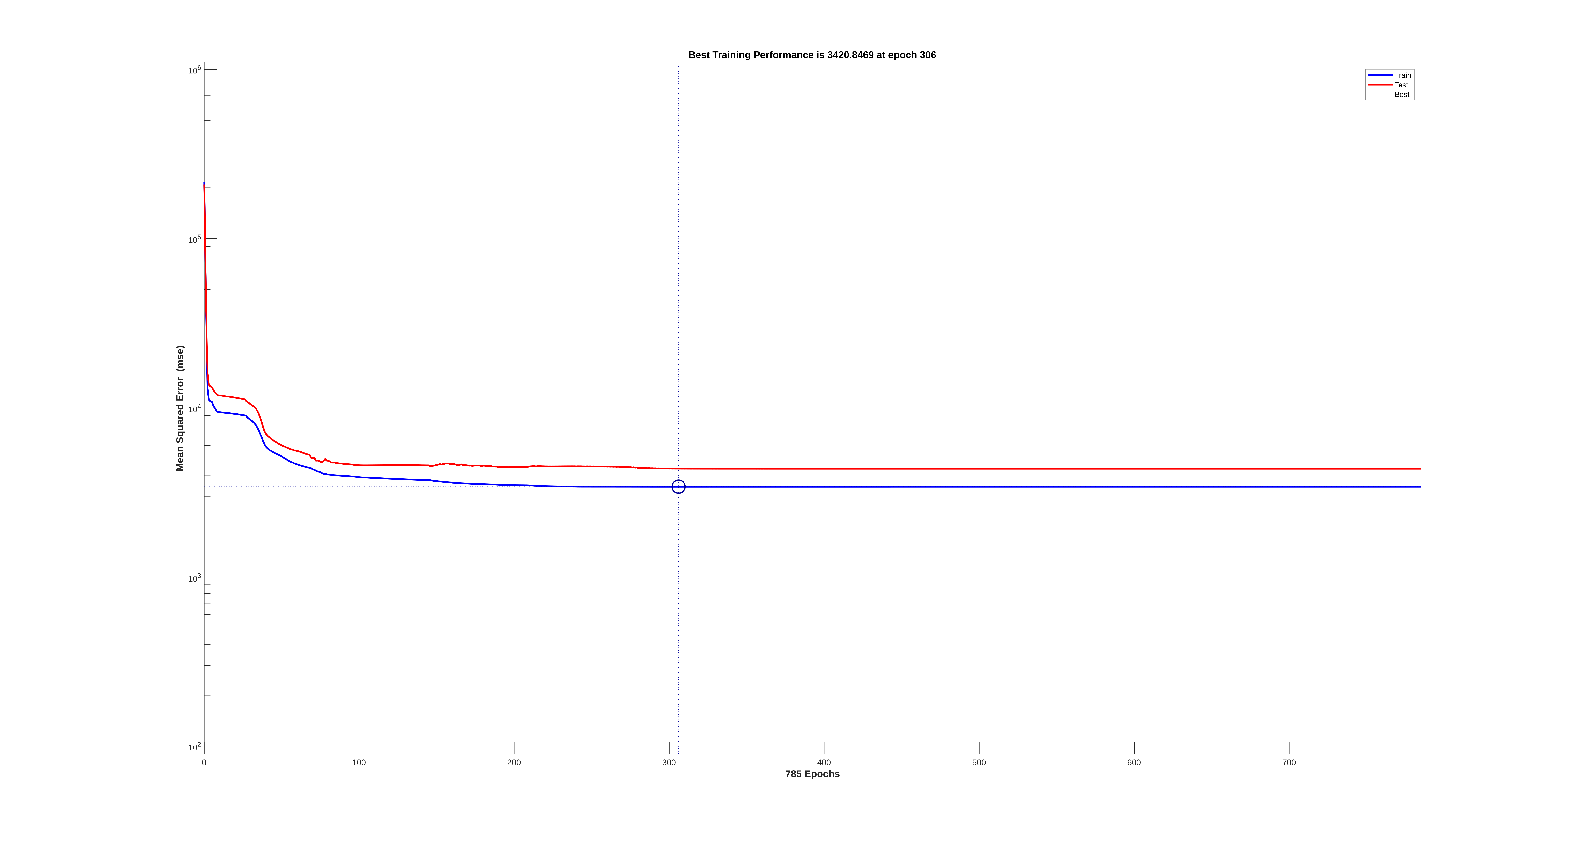
\includegraphics[width=\textwidth, trim=2.95cm 1.1cm 2cm 0.8cm,
		clip]{mlpmeantrainperformance}
		\caption{Training performance plot for the ECG's mean
		estimation network.}\label{fig:mlpmeantrainperformance}
	\end{subfigure}
	\begin{subfigure}{\textwidth}
		\centering
		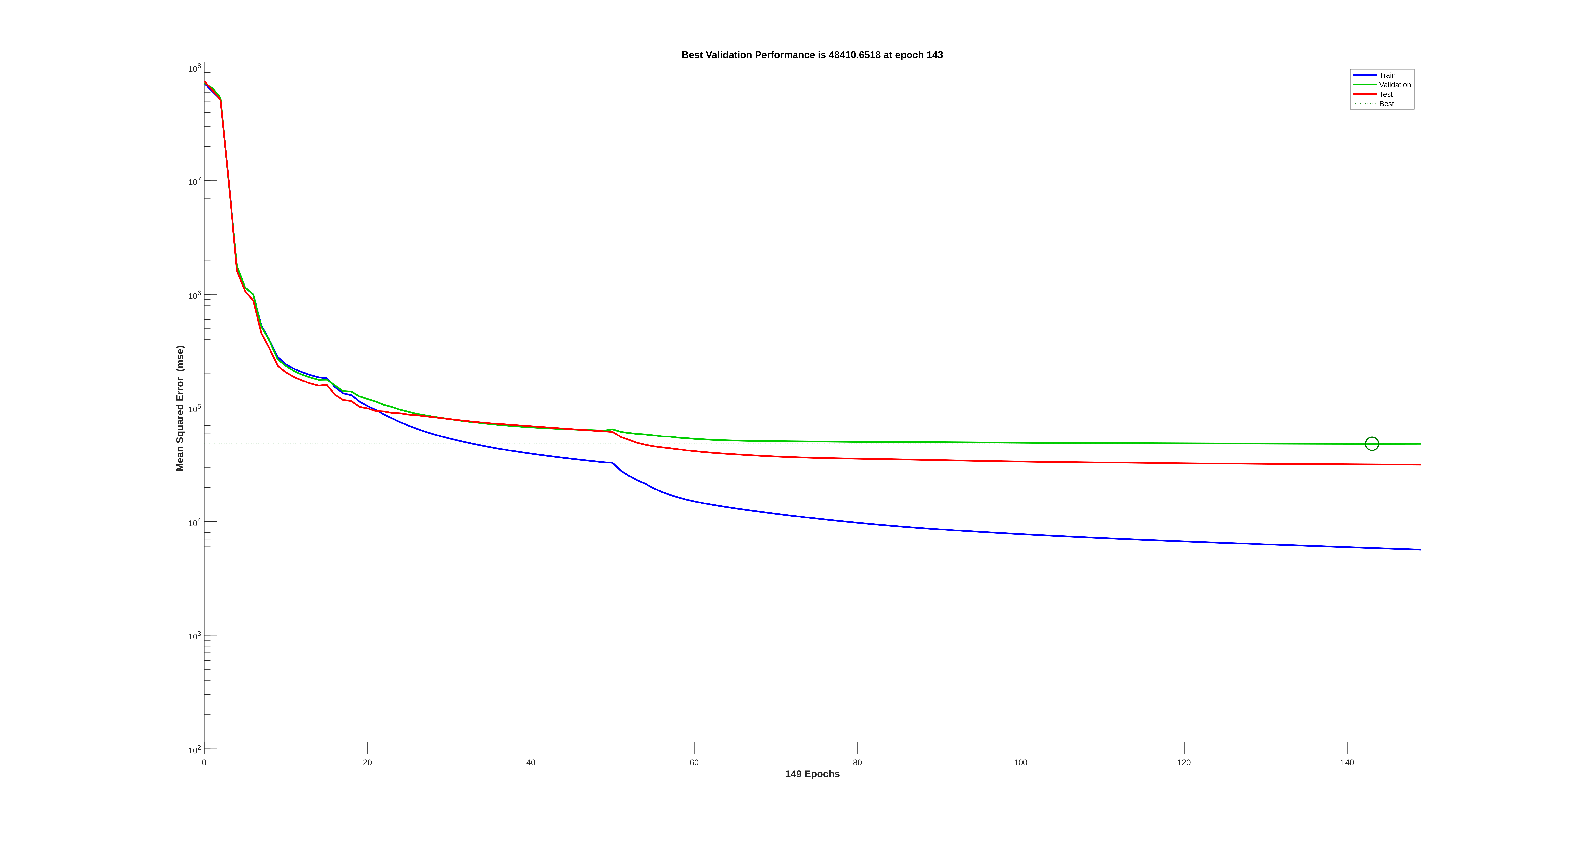
\includegraphics[width=\textwidth, trim=2.95cm 1.1cm 2cm 0.8cm,
		clip]{mlpstdtrainperformance}
		\caption{Training performance plot for the ECG's standard
		deviation estimation network.}\label{fig:mlpstdtrainperformance}
	\end{subfigure}
	\caption{Training performance plots for the two
	networks.}\label{fig:mlptrainperformance}
\end{figure}

\vfigref{fig:mlpstdregression} shows the regression plot for the ECG's standard
deviation estimation network. The network performs very well, with a
coefficient \(R = 0.99184\) for the test set and \(R = 0.99616\) for the entire
dataset.

\begin{figure}[htbp]
	\centering
	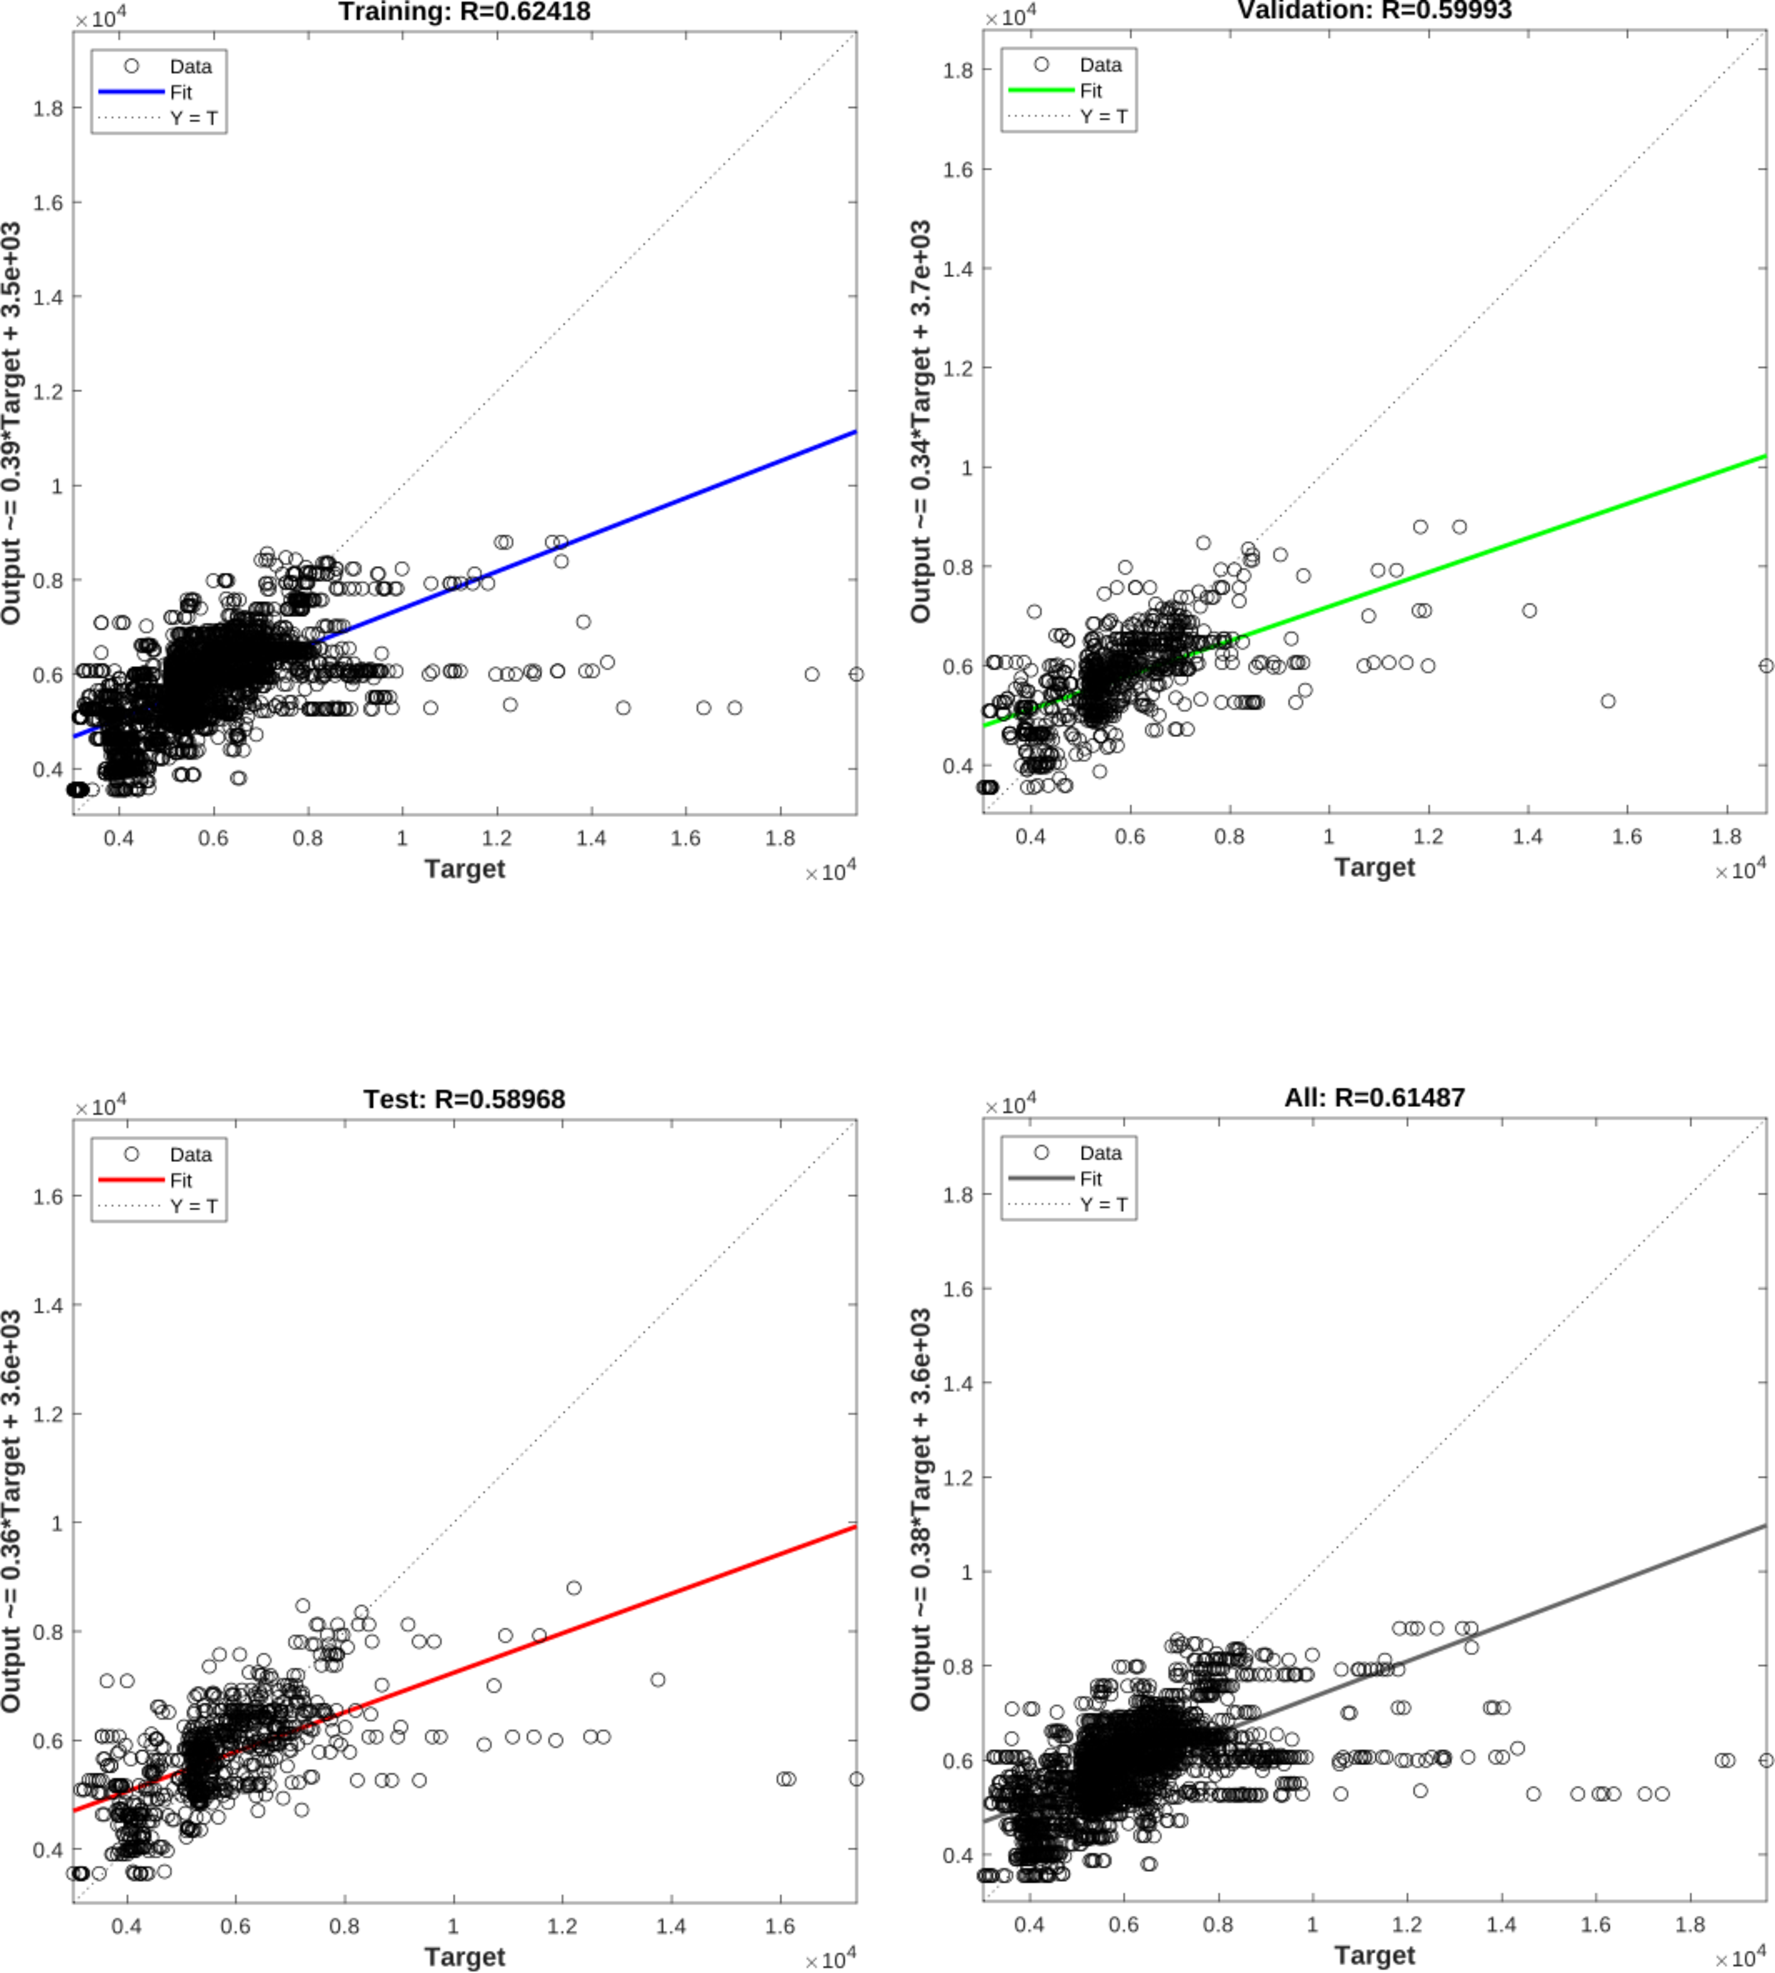
\includegraphics[width=\textwidth]{mlpstdregression}
	\caption{The regression plot for the ECG's standard deviation
	estimation network shows excellent
	results.}\label{fig:mlpstdregression}
\end{figure}

The ECG's mean estimation network performances are not so good (but still
valuable), as shown in \vfigref{fig:mlpmeanregression}: we have \(R = 0.85045\)
for the test set and \(R = 0.85761\) for the entire dataset. This latter
network will be the subject of \chref{ch:cnn}.

\begin{figure}[htbp]
	\centering
	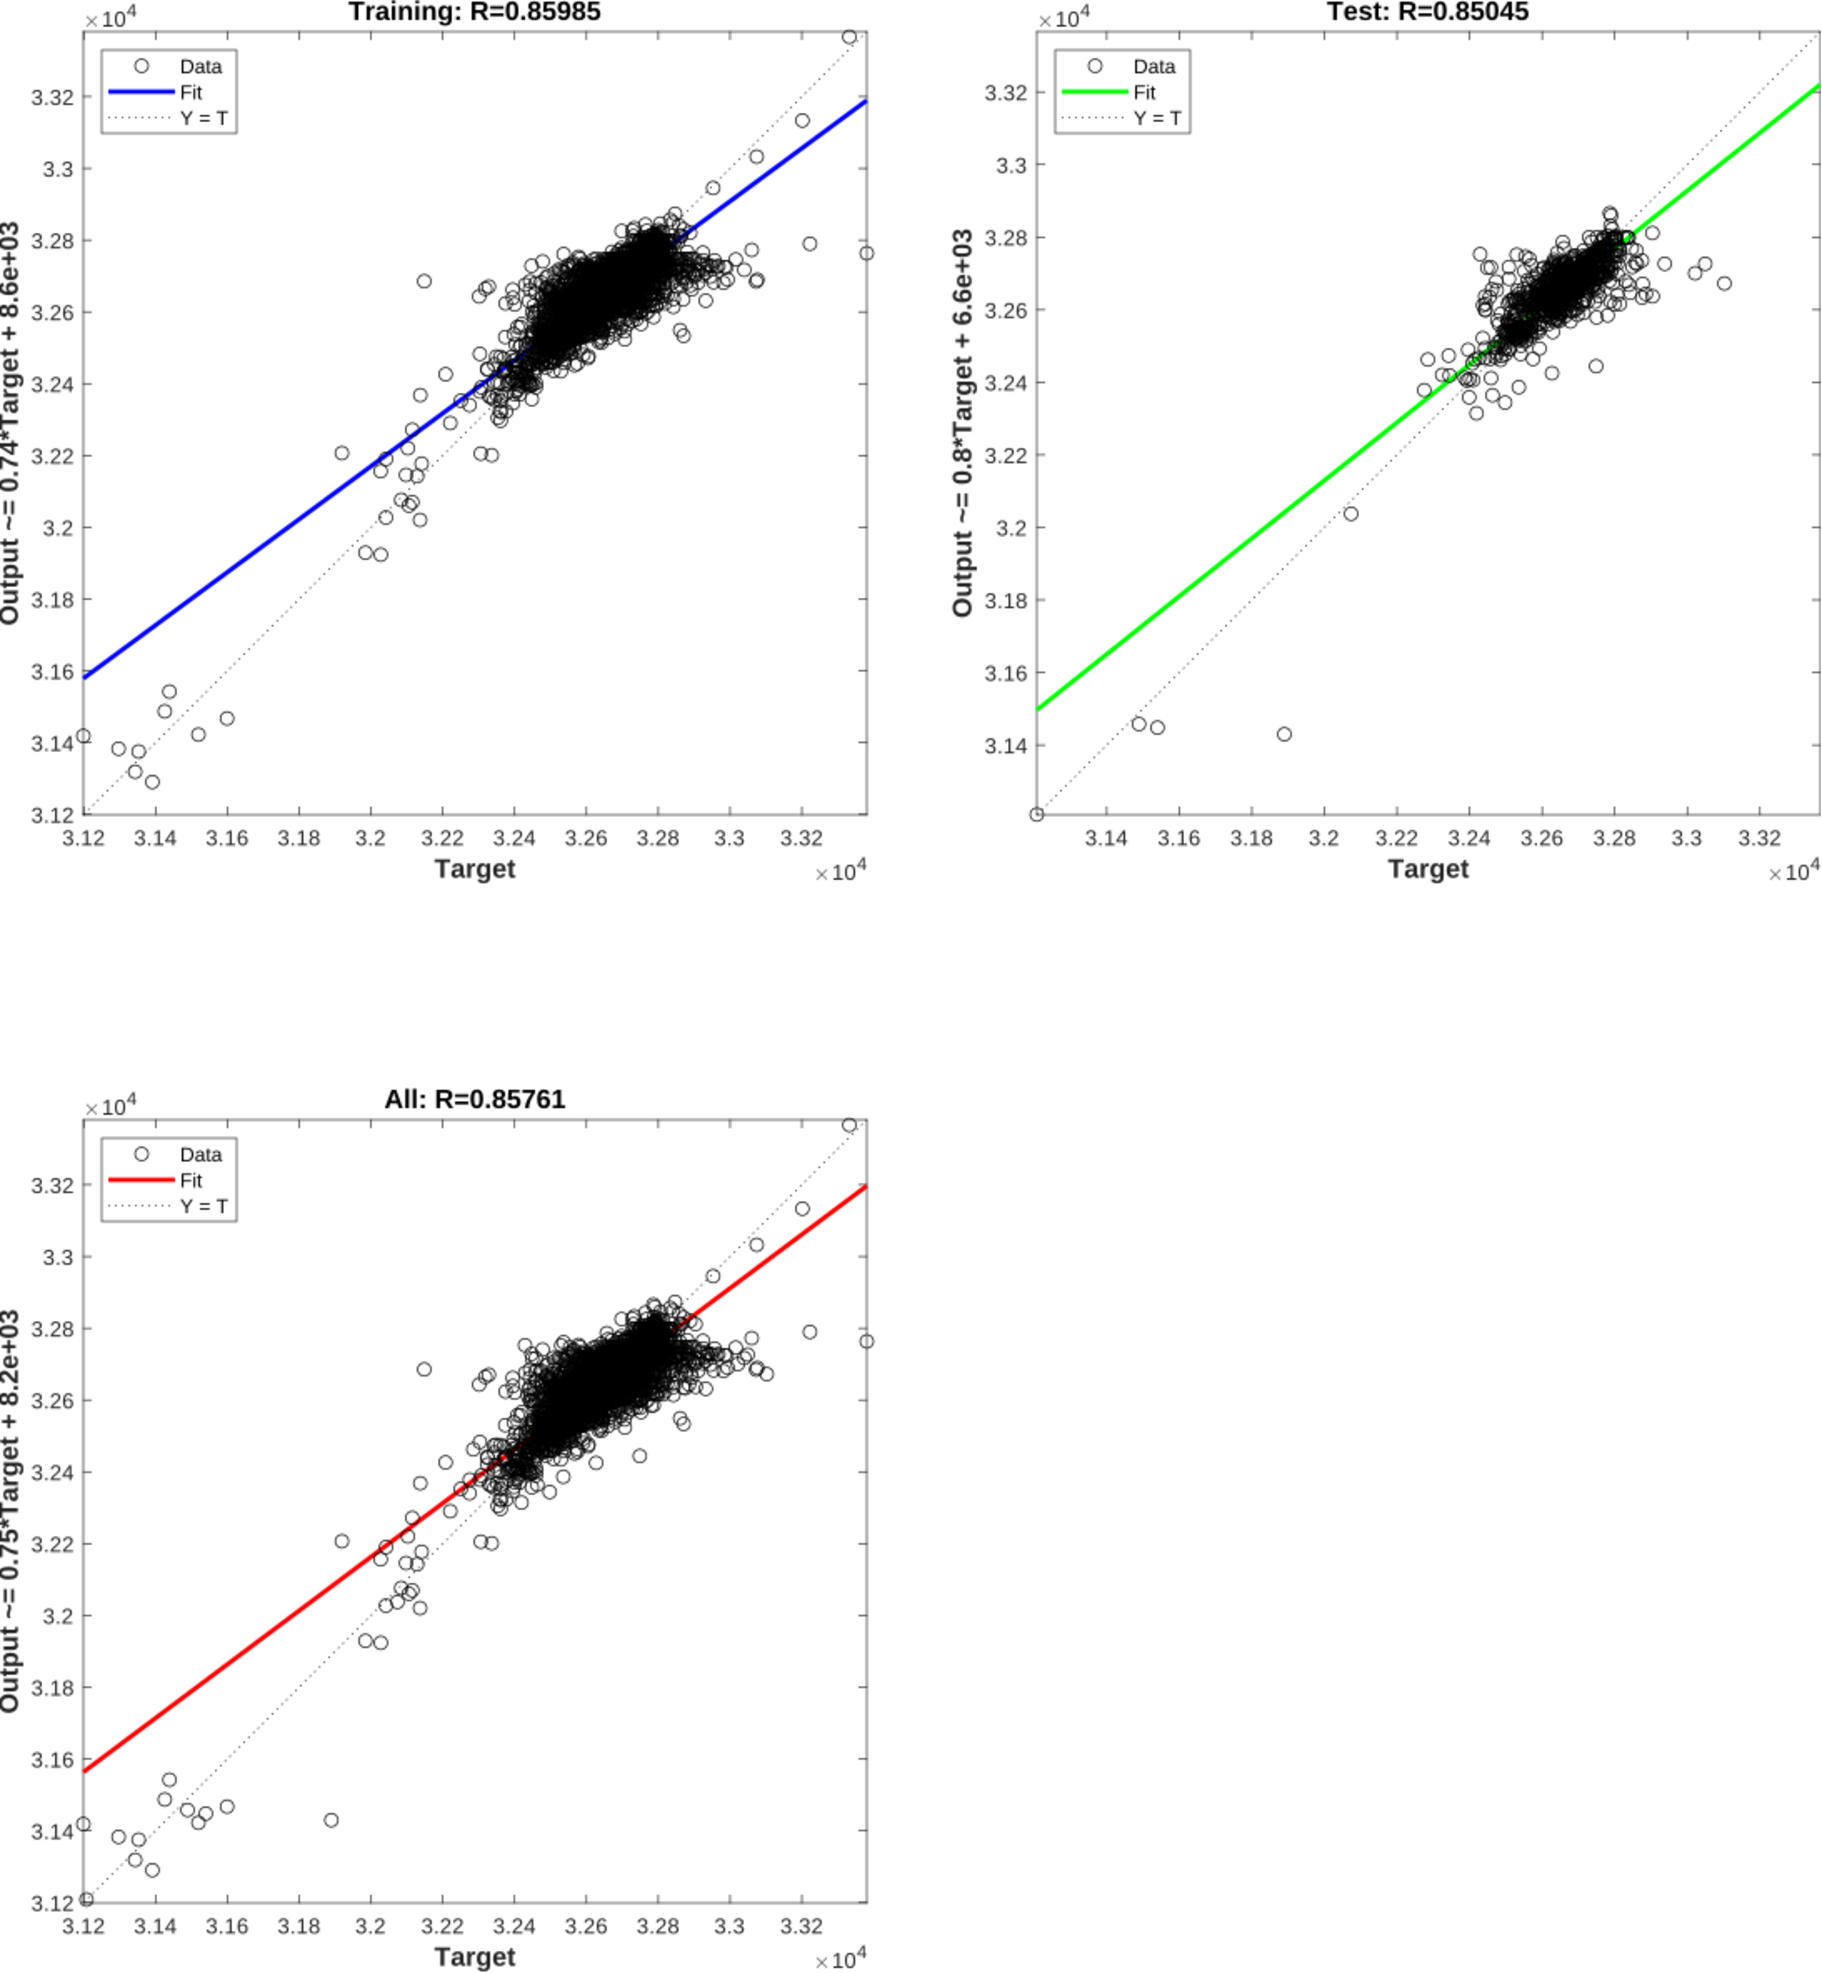
\includegraphics[width=\textwidth]{mlpmeanregression}
	\caption{The regression plot for the ECG's mean estimation network
	shows good, but not excellent, results.}\label{fig:mlpmeanregression}
\end{figure}

\vfigref{fig:mlperrorhists} shows the error histograms for both networks.

\begin{figure}[htbp]
	\centering
	\begin{subfigure}{\textwidth}
		\centering
		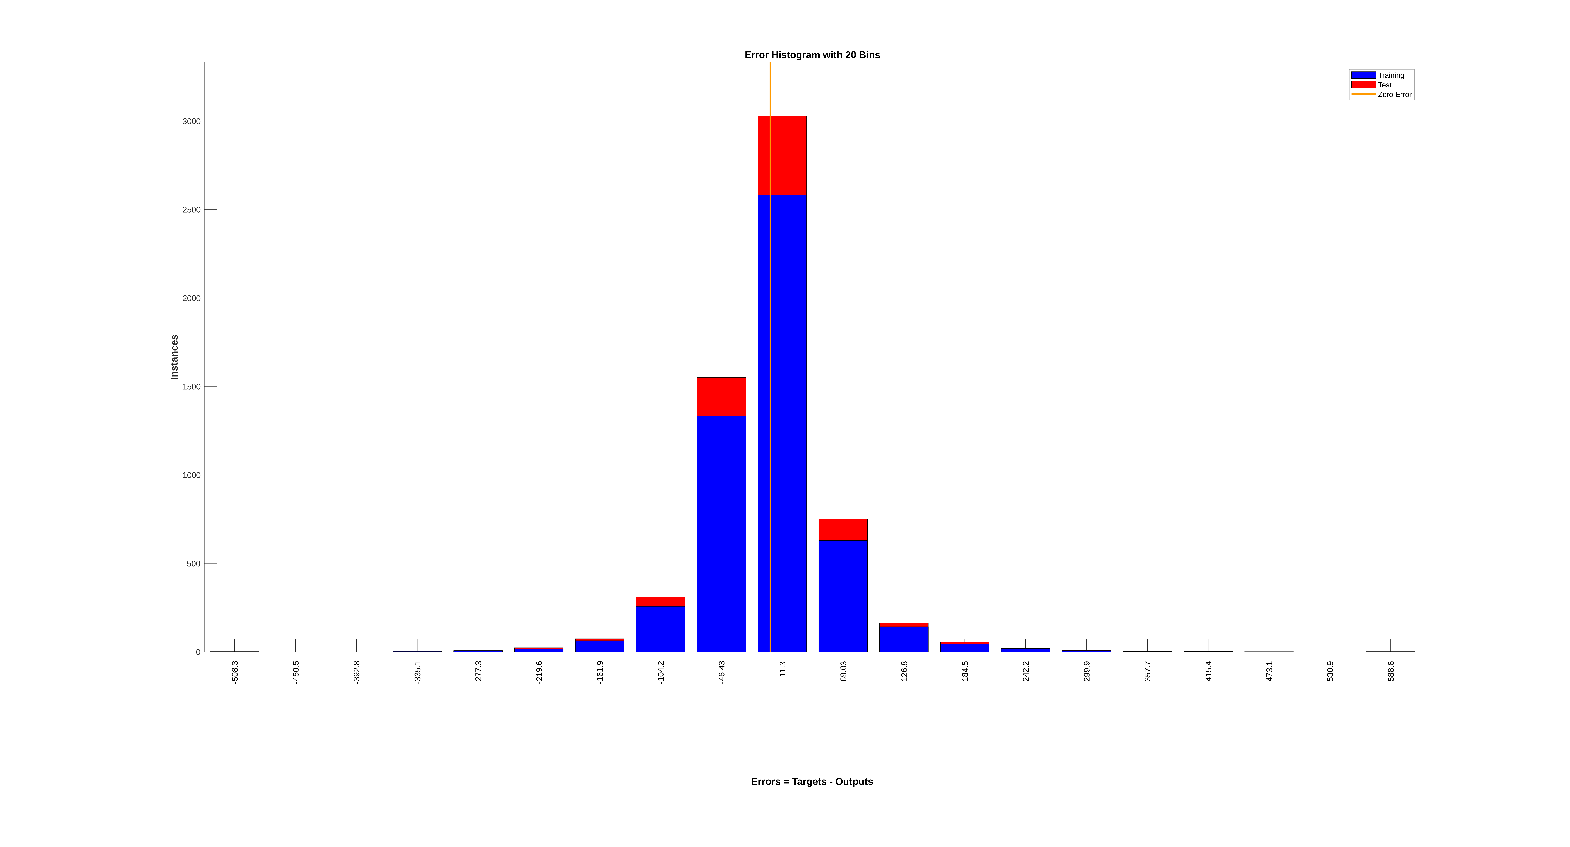
\includegraphics[width=\textwidth, trim=2.9cm 1cm 2cm 0.8cm,
		clip]{mlpmeanerrorhist}
		\caption{Error histogram for the ECG's mean estimation
		network.}\label{fig:mlpmeanerrorhist}
	\end{subfigure}
	\begin{subfigure}{\textwidth}
		\centering
		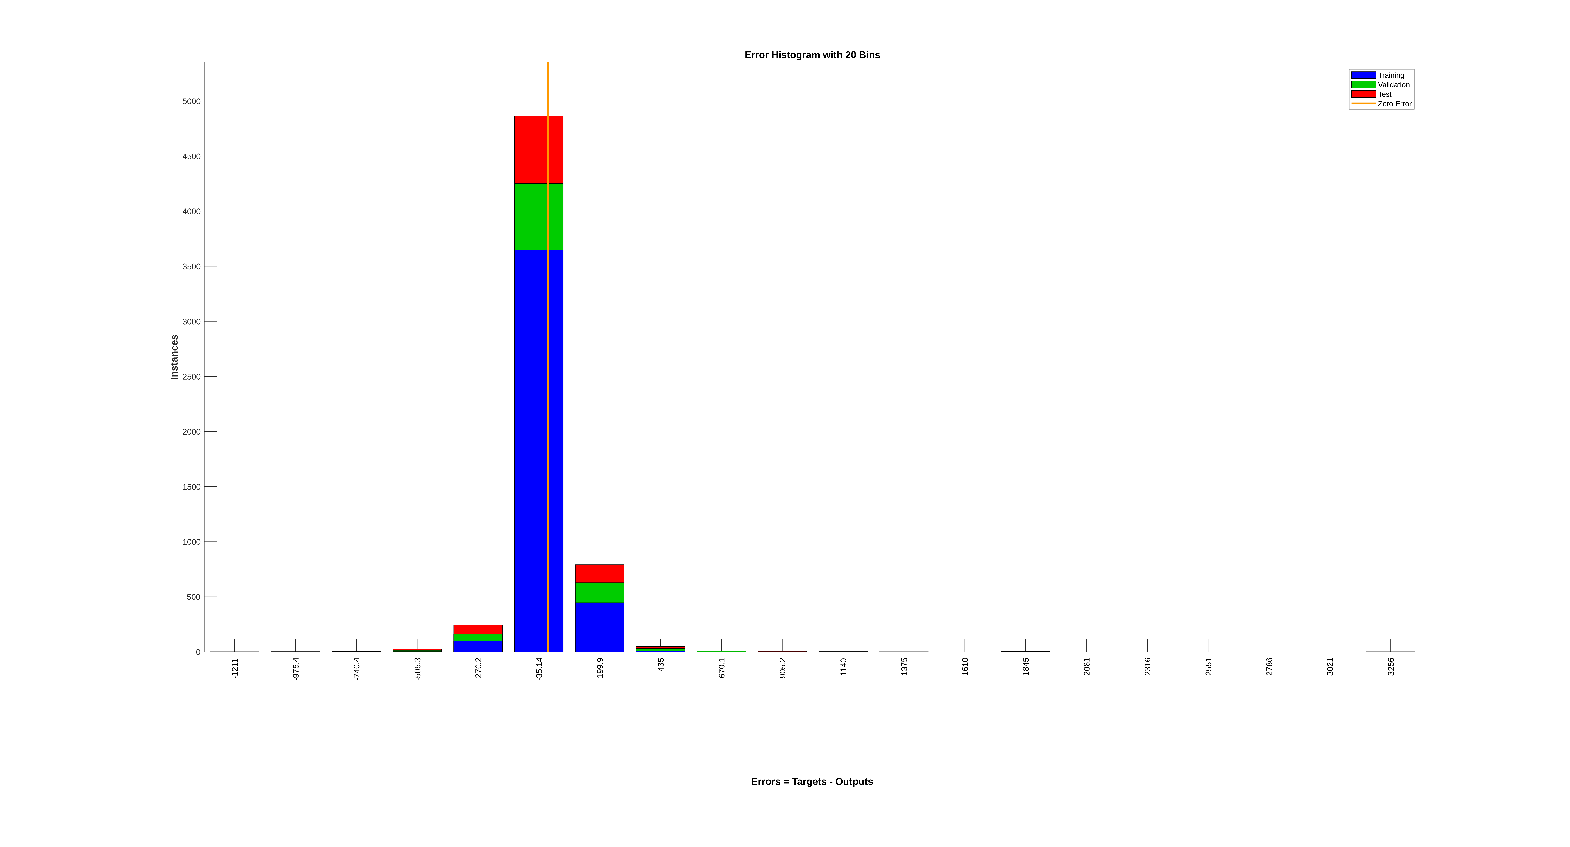
\includegraphics[width=\textwidth, trim=2.9cm 1cm 2cm 0.8cm,
		clip]{mlpstderrorhist}
		\caption{Error histogram for the ECG's standard deviation
		estimation network.}\label{fig:mlpstderrorhist}
	\end{subfigure}
	\caption{Error histograms for the two
	networks.}\label{fig:mlperrorhists}
\end{figure}

\section{Adding a dropout layer}\label{sec:cnndropout}

Finally I'm going to try to add 2 dropout layers between the fully connected
layers. I'll try the following two configurations (only the probability of the
first dropout layer changes):

CNN definition 41:
\begin{verbatim}
fullyConnectedLayer(180)
dropoutLayer(0.2)
fullyConnectedLayer(50)
dropoutLayer(0.1)
fullyConnectedLayer(10)
fullyConnectedLayer(1)
\end{verbatim}

CNN definition 42:
\begin{verbatim}
fullyConnectedLayer(180)
dropoutLayer(0.3)
fullyConnectedLayer(50)
dropoutLayer(0.1)
fullyConnectedLayer(10)
fullyConnectedLayer(1)
\end{verbatim}

The 2 tests are executed in 45 epochs with a validation set (\(15\%\) of
samples) and a validation frequency of 5 iterations.

Results are shown in \tableref{table:cnndropout}. All values are relative to
the best validation loss network.

\begin{table}[hbtp]
	\centering
	\begin{tabular}{|c|c|c|c|c|c|}
		\toprule
		\# & Dropout & Tr.~RMSE & Val.~RMSE & Tr.~R & Val.~R \\
		\midrule
		41 & \(0.2\) & \(678.59\) & \(490.41\) & \(0.945\) & \(0.936\) \\
		42 & \(0.3\) & \(640.06\) & \(560.28\) & \(0.950\) & \(0.929\) \\
		\bottomrule
	\end{tabular}
	\caption{Adding dropout layers to avoid
	overfitting.}\label{table:cnndropout}
\end{table}

As the objective is to avoid overfitting, I will use a dropout probability of
\(0.2\) as the \(R\) values for training and validation sets are more similar.

\section{Final Convolutional Neural Network}\label{sec:cnnfinalcnn}

The final CNN is shown in \lstref{lst:finalcnn} and available in the definition
file named \code{cnndef.m}.

\lstinputlisting[language={matlab}, label={lst:finalcnn},
style={Matlab-editor}, basicstyle={\footnotesize\ttfamily}, caption={The final
CNN architecture and training options.}]{cnndef.m}

This network has been trained with 200 epochs. Samples were divided as follows:
\begin{itemize}
\item Training set: \(70\%\) (\(4200\) samples).
\item Validation set: \(15\%\) (\(900\) samples).
\item Test set: \(15\%\) (\(900\) samples).
\end{itemize}

A test set has been used since the validation set is used to select the output
network of the training process. So the test set allows for an unbiased
evaluation of the performance of the network.

Training ended after 3952 iterations (112 epochs plus some iterations), due to
validation loss not improving anymore. Complete results are shown in
\lstref{lst:cnnresults}. \figref{fig:cnnregression} shows the regression plots
for the CNN. The CNN clearly outperformed the MLP developed in \chref{ch:ecg}.

\lstinputlisting[language={}, label={lst:cnnresults},
caption={Results of the final Convolutional Neural Network.}]{cnnresults.txt}

\begin{figure}[htbp]
	\centering
	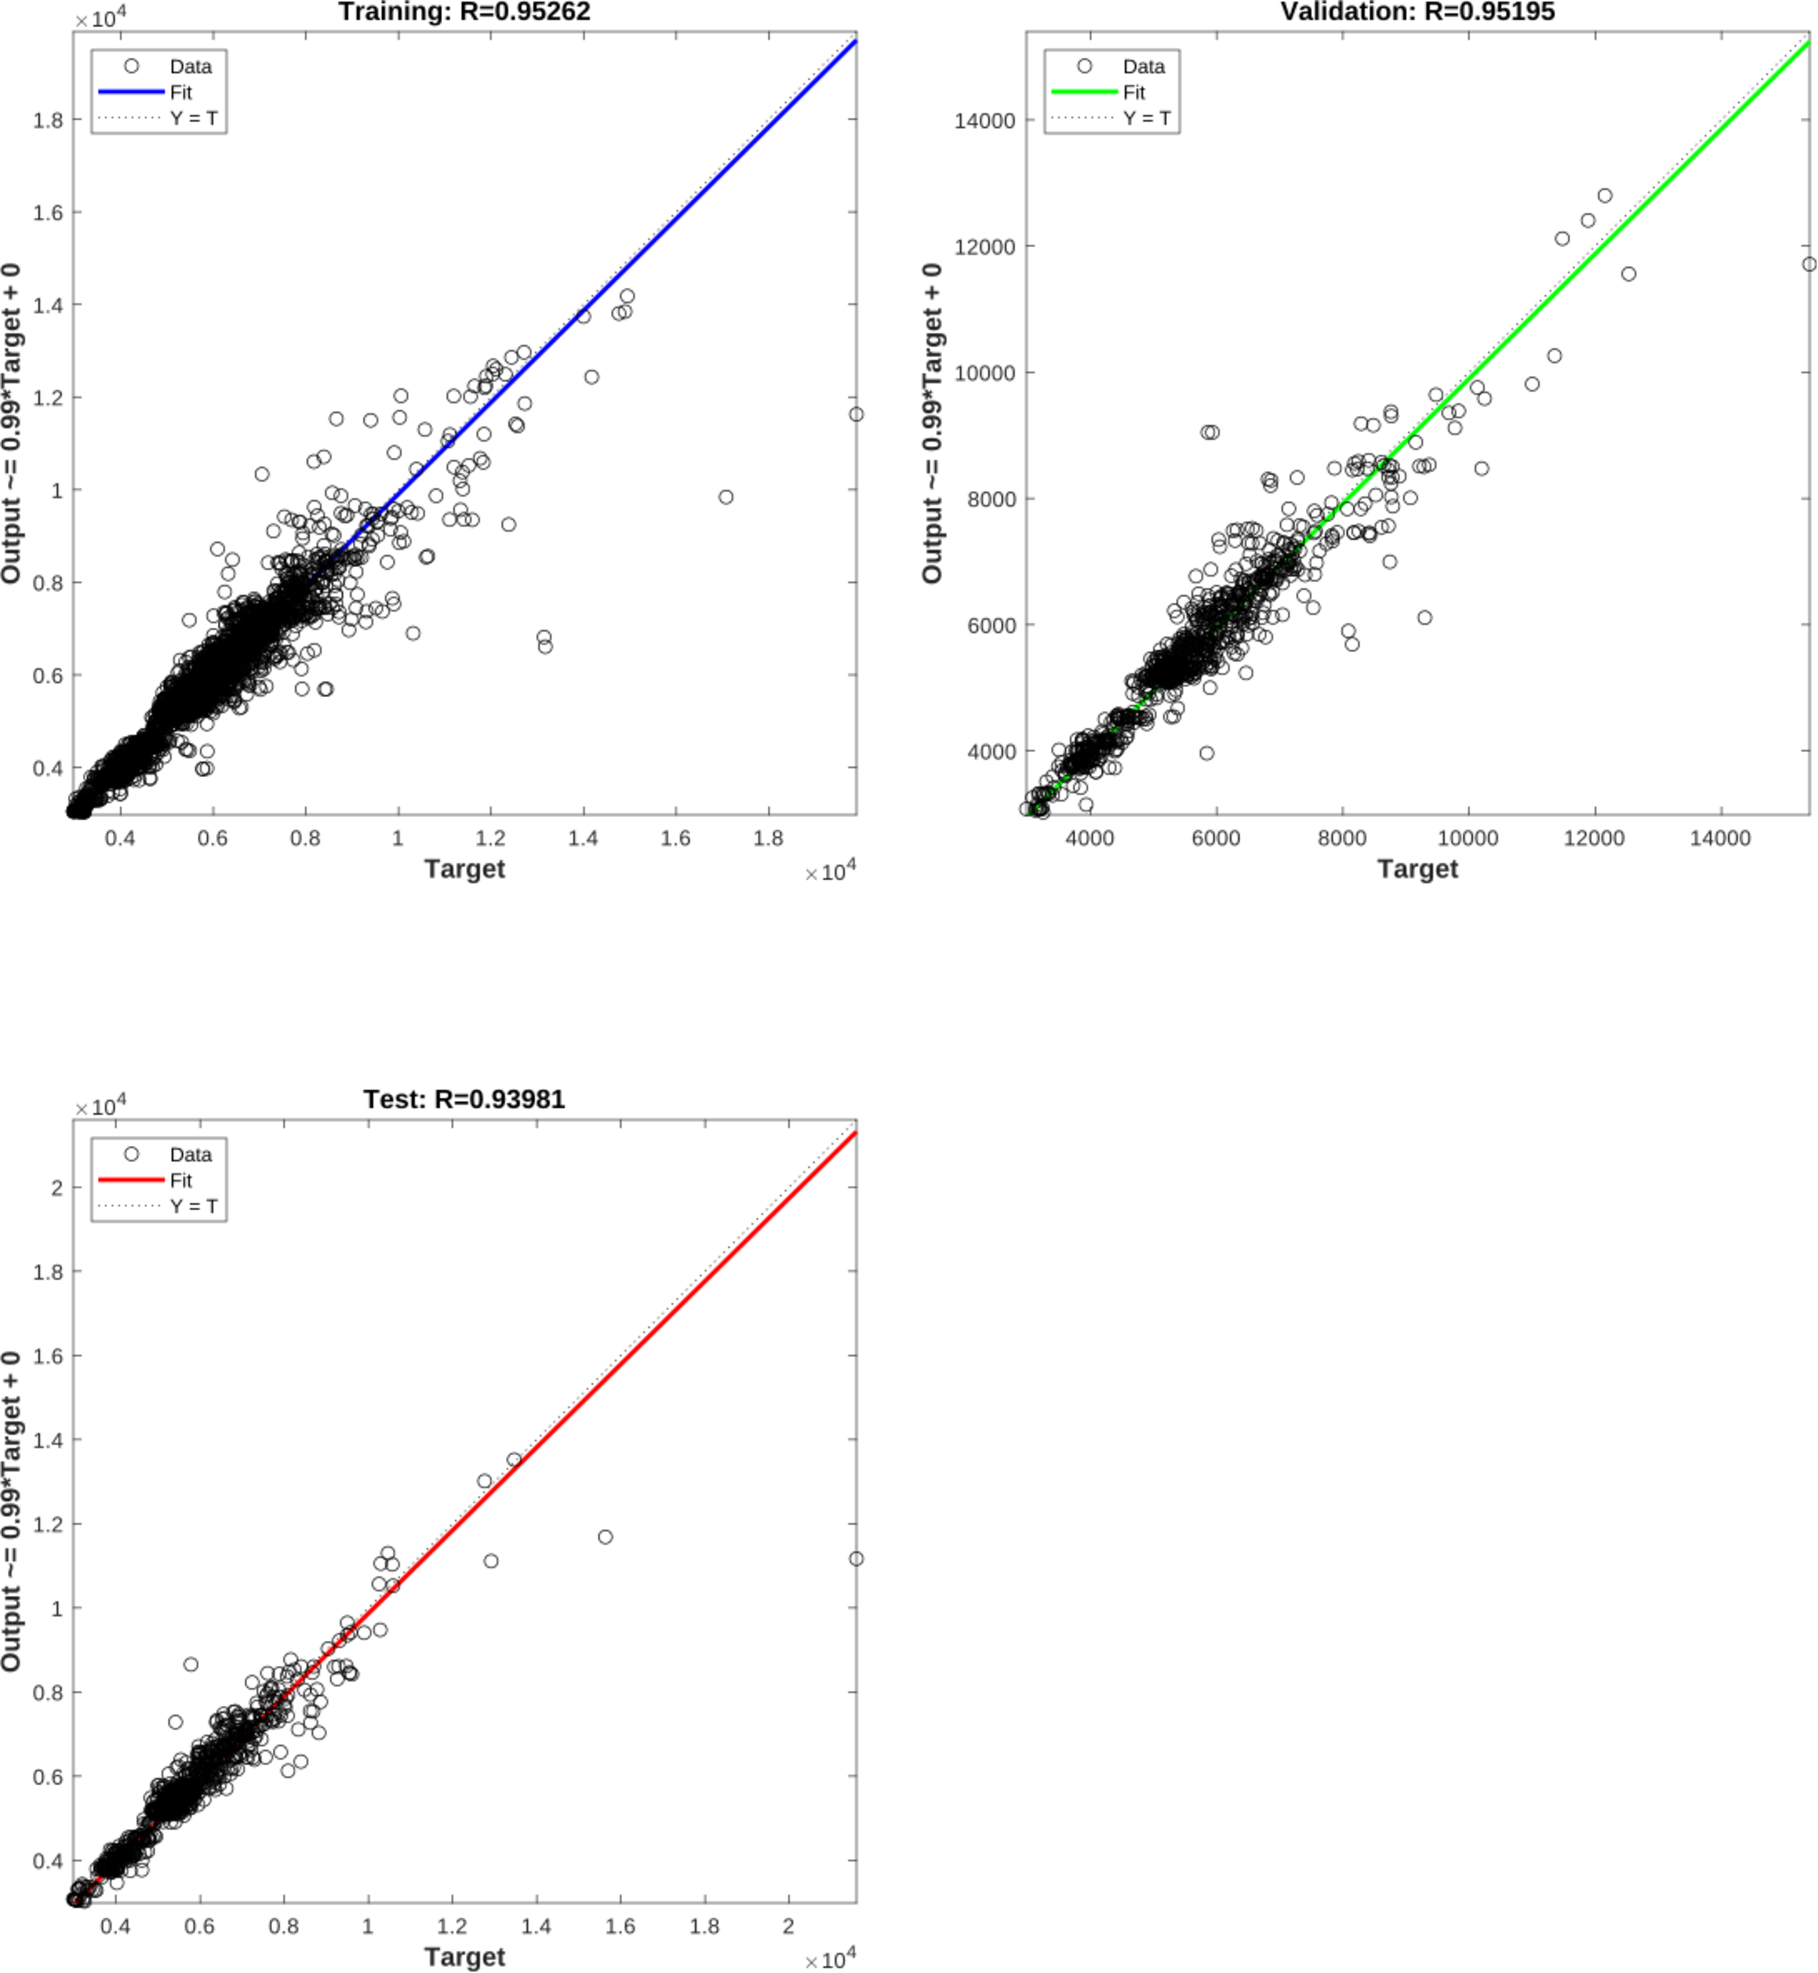
\includegraphics[width=\textwidth]{cnnregression}
	\caption{Regression plots for all three sets for the Convolutional
	Neural Network doing the task of estimating the ECG's standard
	deviation.}\label{fig:cnnregression}
\end{figure}

